\section{Cải tiến mô hình}
\subsection{Mô hình 1 - CNN}
\subsubsection{Dữ liệu đầu vào }
Mô hình này sẽ có đầu vào là bộ dữ liệu \textbf{Fashion Product Images (Small)} đã được xử lý với 41906 hình ảnh cho 3 lớp.\\

Sử dụng \textbf{ImageDataGenerator} chia dữ liệu thành 2 tập là training\_generator và validation\_generator, đồng thời tăng cường thêm dữ liệu như sau:
\begin{lstlisting}
from keras.preprocessing.image import ImageDataGenerator

#image generator object from keras. reference : Keras Docs
image_generator = ImageDataGenerator(
    validation_split=0.2, 
    rescale=1/255, 
    shear_range = 0.2, 
    zoom_range = 0.2, 
    horizontal_flip = True
)

#create a flow of images for training the model.
training_generator = image_generator.flow_from_dataframe(
    dataframe = df,
    directory= "/content/drive/MyDrive/myntradataset/images/",
    x_col="image",
    y_col="masterCategory",
    target_size=(224,224),
    batch_size=32,
    subset="training"

)

#create a flow of images for validating(testing) the trained model.
validation_generator = image_generator.flow_from_dataframe(
    dataframe = df,
    directory="/content/drive/MyDrive/myntradataset/images/",
    x_col="image",
    y_col="masterCategory",
    target_size=(224,224),
    batch_size=32,
    subset="validation"
)
\end{lstlisting}
Found 33525 validated image filenames belonging to 3 classes.\\
Found 8381 validated image filenames belonging to 3 classes.\\

\newpage
Còn tập test sẽ đc lấy ra một phần từ tập validation\_generator như sau:
\begin{lstlisting}
batch_size = 32
#!pip install tqdm
import tqdm
validation_generator.reset()
X_test, y_test = next(validation_generator)
for i in tqdm.tqdm(range(int(validation_generator.n/batch_size)-200)): 
  img, label = next(validation_generator)
  X_test = np.append(X_test, img, axis=0 )
  y_test = np.append(y_test, label, axis=0)
print(X_test.shape, y_test.shape)
\end{lstlisting}
Thu được tập test gồm có 1984 hình ảnh và nhãn của nó.

\subsubsection{Xây dựng mô hình}
%So với mô hình 1 thì mô hình thứ 2 này tuy vẫn dùng CNN nhưng cấu trúc nó thì được thay đổi, kể cả việc đưa dữ liệu đầu vào cũng đc xử lý theo một cách khác với target\_size là 224
\begin{lstlisting}
from keras import layers,models
model1 = Sequential()
model1.add(layers.Conv2D(16, (4,4),  activation = 'relu' , input_shape = (224,224,3)))
model1.add(MaxPooling2D(pool_size = (2, 2)))

model1.add(Conv2D(32, (3,3), activation='relu'))
model1.add(MaxPooling2D(pool_size = (2, 2)))

model1.add(Conv2D(64, (3,3), activation='relu'))
model1.add(MaxPooling2D(pool_size = (2, 2)))

model1.add(Conv2D(64, (3,3), activation='relu'))
model1.add(MaxPooling2D(pool_size = (2, 2)))

model1.add(Conv2D(128, (3,3), activation='relu'))
model1.add(MaxPooling2D(pool_size = (2, 2)))


model1.add(Flatten())
model1.add(Dense(units=512, activation='relu'))
model1.add(Dropout(0.25))
model1.add(Dense(units=256, activation='relu'))
model1.add(Dropout(0.25))
model1.add(Dense(units=128, activation='relu'))
model1.add(Dropout(0.25))
model1.add(Dense(units=3, activation='softmax'))

model1.compile(optimizer='adam',
              loss='categorical_crossentropy',
              metrics=['accuracy'])

model1.summary()
\end{lstlisting}
\newpage
\begin{center}
    \begin{figure}[!h]
        \centering
        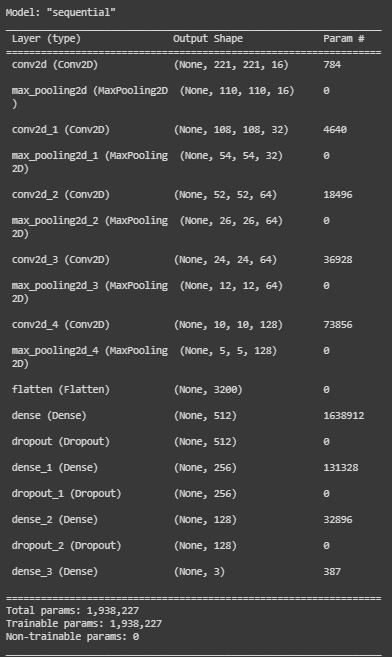
\includegraphics[scale = 1.2]{fileanh/13.jpg}
        \caption{Model CNN}
    \end{figure}
\end{center}
\subsubsection{Kết quả training}
\begin{center}
    \begin{figure}[!h]
        \centering
        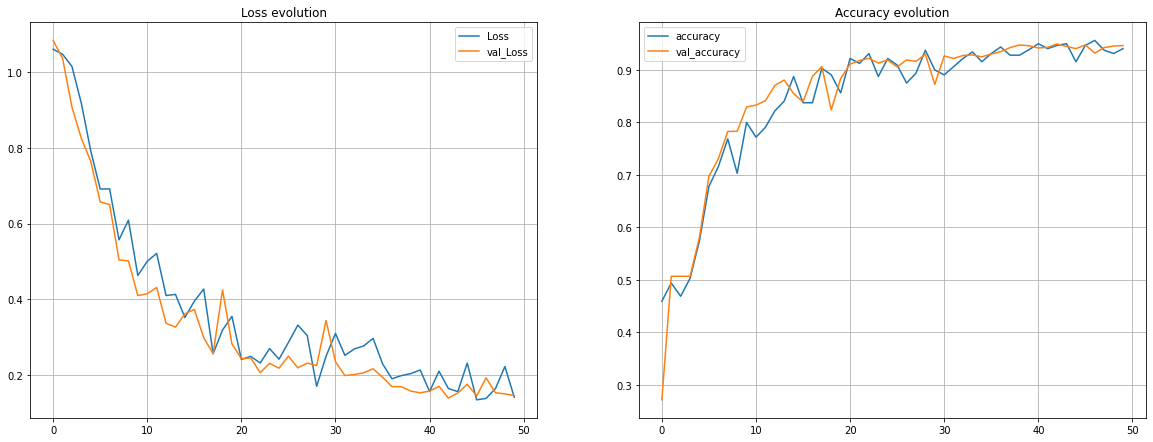
\includegraphics[scale = 0.38]{fileanh/17.png}
        \caption{Kết quả train của Model CNN}
    \end{figure}
\end{center}
\subsubsection{Đánh giá}
Ta có ma trận nhầm lẫn như sau:
\begin{center}
    \begin{figure}[!h]
        \centering
        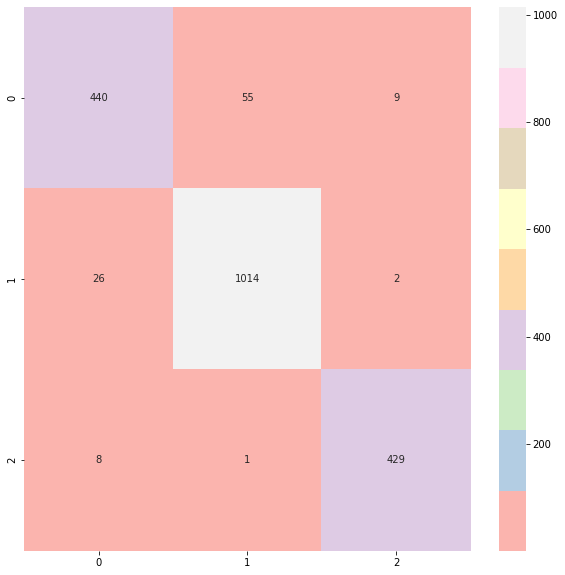
\includegraphics[scale = 0.4]{fileanh/18.png}
        \caption{Confusion matrix của Model CNN}
    \end{figure}
\end{center}
Và các giá trị Macro average Precision, Macro average Recall, F1-score là:
\begin{center}
    \begin{figure}[!h]
        \centering
        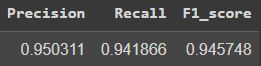
\includegraphics[scale = 1.6]{fileanh/19.jpg}
        \caption{Các chỉ số đánh giá của Model CNN}
    \end{figure}
\end{center}


\subsection{Mô hình 2 - CNN với tập dữ liệu lớn}
Sử dụng mô hình CNN đã được xây dựng trước đó, thực hiện training với tập dữ liệu lớn hơn.
\subsubsection{Dữ liệu đầu vào }
\begin{itemize}
    \item Mô hình này sẽ có đầu vào là bộ dữ liệu đã được tăng cường hình ảnh từ nhiều nguồn khác với tất cả 79596 hình ảnh cho 3 lớp.

    \item Sử dụng \textbf{ImageDataGenerator} thực hiện tăng cường và chia dữ liệu thành các tập train, test và validation với số lượng ảnh gốc (chưa được tăng cường ví dụ như xoay ảnh,..):
    \begin{itemize}
        \item train : 63677 hình ảnh
        \item validation : 15919 hình ảnh
        \item test : 3136 hình ảnh
    \end{itemize}
\end{itemize}

\subsubsection{Kết quả training}
\begin{center}
    \begin{figure}[!h]
        \centering
        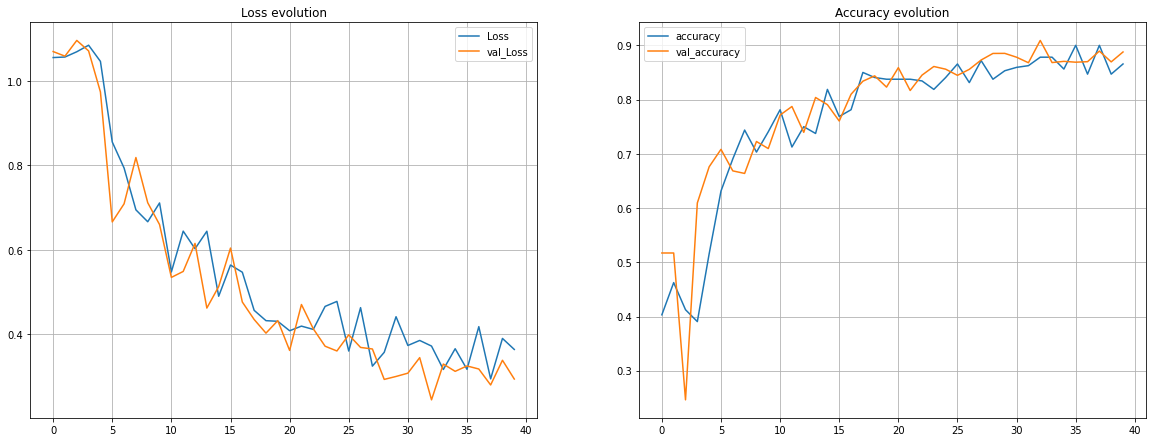
\includegraphics[scale = 0.38]{fileanh/CNNtc.png}
        \caption{Kết quả train của Model CNN với tập dữ liệu lớn}
    \end{figure}
\end{center}
\subsubsection{Đánh giá}
Ta có ma trận nhầm lẫn như sau:
\begin{center}
    \begin{figure}[!h]
        \centering
        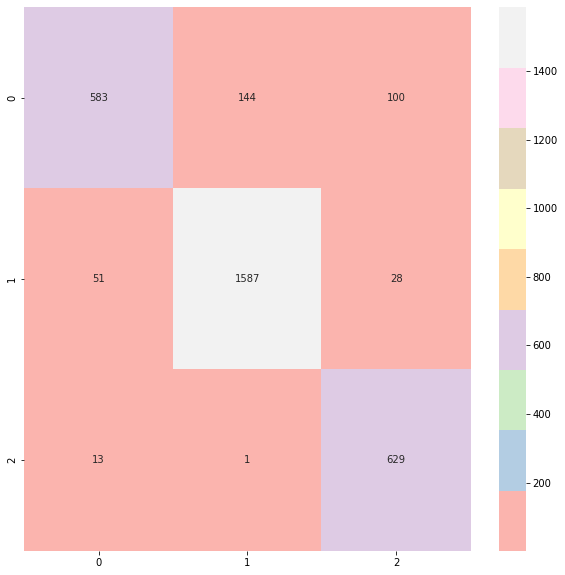
\includegraphics[scale = 0.42]{fileanh/CNNtc1.png}
        \caption{Confusion matrix của Model CNN với tập dữ liệu lớn}
    \end{figure}
\end{center}
\newpage
Và các giá trị Macro average Precision, Macro average Recall, F1-score là:
\begin{center}
    \begin{figure}[!h]
        \centering
        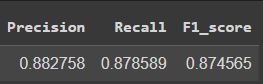
\includegraphics[scale = 1.5]{fileanh/CNNtc2.jpg}
        \caption{Các chỉ số đánh giá của Model CNN với tập dữ liệu lớn}
    \end{figure}
\end{center}

\subsection{Mô hình 3 - VGG16}
\subsubsection{Dữ liệu đầu vào}
Bộ dữ liệu \textbf{Fashion Product Images (Small)} đã được xử lý với 41906 hình ảnh cho 3 lớp.
\subsubsection{Xây dựng mô hình}
\begin{lstlisting}
image_size=[227,227]
model=VGG16(input_shape=image_size+[3],include_top=False,weights="imagenet")
\end{lstlisting}
\begin{lstlisting}
for layers in model.layers:
  layers.trainable=False
\end{lstlisting}
Thêm một số layers cần thiết
\begin{lstlisting}
final_model=Model(inputs=model.input,outputs=Dense(3,activation="softmax")(Flatten()(model.output)))
final_model.summary()
\end{lstlisting}
\begin{lstlisting}
final_model.compile(loss="binary_crossentropy",optimizer="adam",metrics=['accuracy'])  
vgg16=final_model.fit(training_generator,epochs=50,steps_per_epoch=20,validation_data=validation_generator)
\end{lstlisting}
\newpage
\begin{center}
    \begin{figure}[!h]
        \centering
        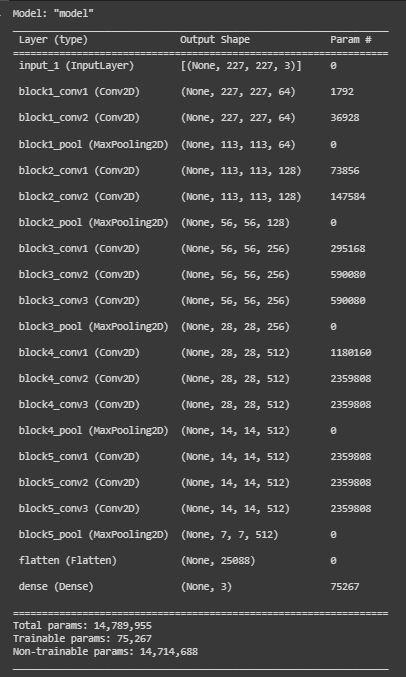
\includegraphics[scale = 1]{fileanh/20.jpg}
        \caption{Model VGG16}
    \end{figure}
\end{center}
\subsubsection{Kết quả training}
\begin{center}
    \begin{figure}[!h]
        \centering
        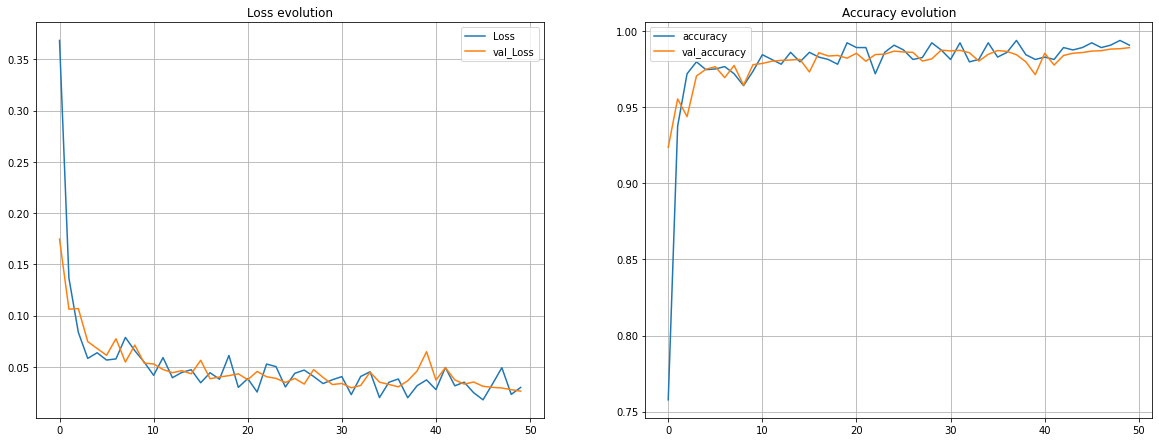
\includegraphics[scale = 0.38]{fileanh/23.png}
        \caption{kết quả train của Model VGG16}
    \end{figure}
\end{center}\newpage
\subsubsection{Đánh giá}
Các giá trị trên ma trận nhầm lẫn:

\begin{center}
    \begin{figure}[!h]
        \centering
        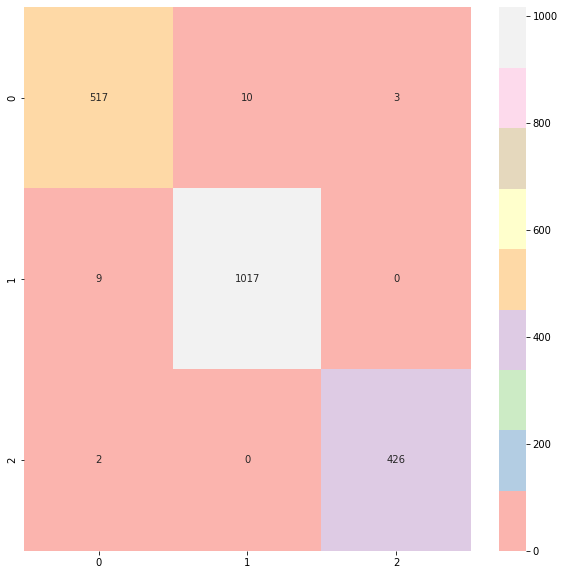
\includegraphics[scale = 0.42]{fileanh/24.png}
        \caption{Confusion matrix của Model VGG16}
    \end{figure}
\end{center}
Và các giá trị Macro average Precision, Macro average Recall, F1-score là:
\begin{center}
    \begin{figure}[!h]
        \centering
        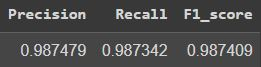
\includegraphics[scale = 1.5]{fileanh/25.jpg}
        \caption{Chỉ số đánh giá của Model VGG16}
    \end{figure}
\end{center}

\subsection{Mô hình 4 - VGG16 với tập dữ liệu lớn}
Sử dụng mô hình VGG16 đã được xây dựng trước đó, thực hiện training với tập dữ liệu lớn hơn.
\subsubsection{Dữ liệu đầu vào }
Bộ dữ liệu đã được tăng cường hình ảnh từ nhiều nguồn khác với tất cả 79596 hình ảnh cho 3 lớp.

\subsubsection{Kết quả training}\newpage
\begin{center}
    \begin{figure}[!h]
        \centering
        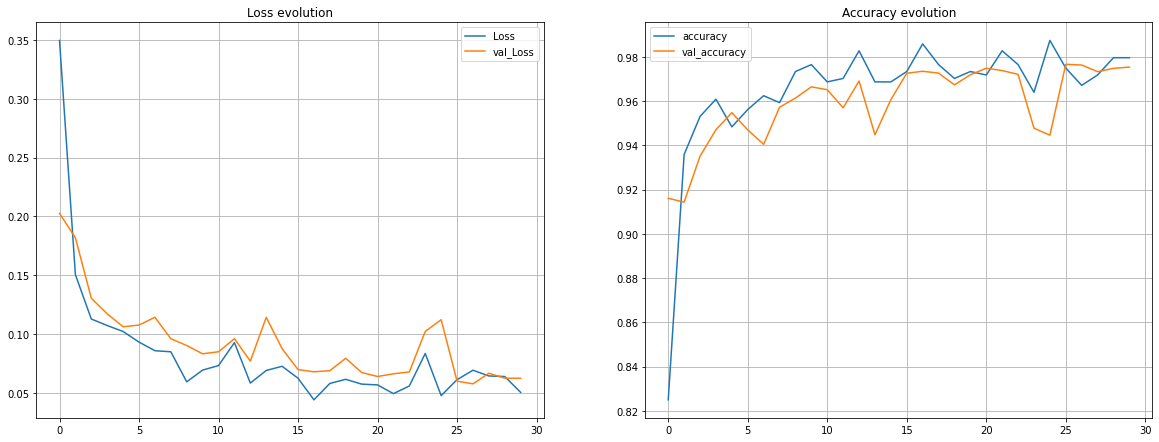
\includegraphics[scale = 0.38]{fileanh/vgg16_increase.png}
        \caption{Kết quả train của Model VGG16 với tập dữ liệu lớn}
    \end{figure}
\end{center}
\subsubsection{Đánh giá}
Ta có ma trận nhầm lẫn như sau:
\begin{center}
    \begin{figure}[!h]
        \centering
        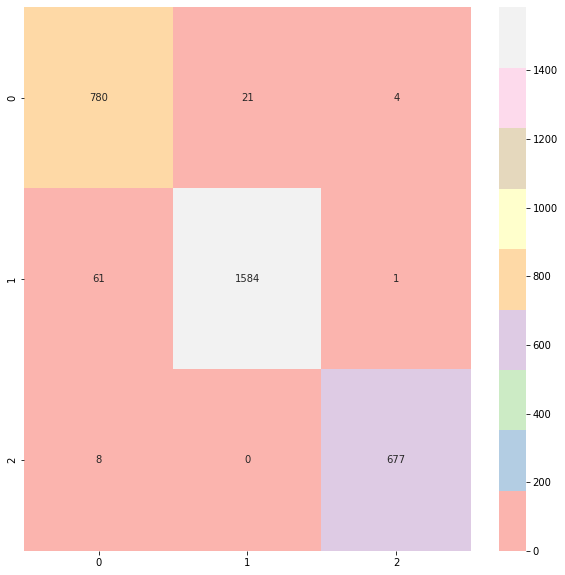
\includegraphics[scale = 0.39]{fileanh/vgg16_increase1.png}
        \caption{Confusion matrix của Model VGG16 với tập dữ liệu lớn}
    \end{figure}
\end{center}

Và các giá trị Macro average Precision, Macro average Recall, F1-score là:
\begin{center}
    \begin{figure}[!h]
        \centering
        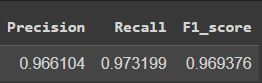
\includegraphics[scale = 1.2]{fileanh/vgg16_increase2.jpg}
        \caption{Các chỉ số đánh giá của Model VGG16 với tập dữ liệu lớn}
    \end{figure}
\end{center}


\subsection{Mô hình 5 - VGG19}
\subsubsection{Dữ liệu đầu vào}
Bộ dữ liệu \textbf{Fashion Product Images (Small)} đã được xử lý với 41906 hình ảnh cho 3 lớp.
\subsubsection{Xây dựng mô hình}
\begin{lstlisting}
image_size=[227,227]
model1=VGG19(input_shape=image_size+[3],include_top=False,weights="imagenet")
\end{lstlisting}
\begin{lstlisting}
for layers in model1.layers:
  layers.trainable=False
\end{lstlisting}
Thêm một số layers cần thiết
\begin{lstlisting}
final_model1=Model(inputs=model1.input,outputs=Dense(3,activation="softmax")(Flatten()(model1.output)))
final_model1.summary()
\end{lstlisting}

\begin{center}
    \begin{figure}[!h]
        \centering
        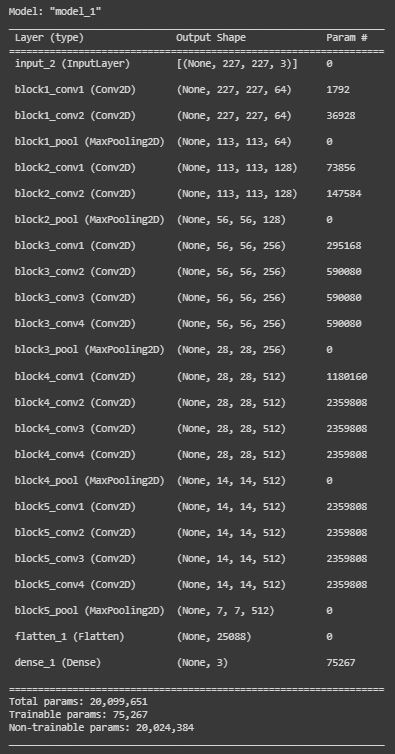
\includegraphics[scale = 1]{fileanh/26.jpg}
        \caption{Model VGG19}
    \end{figure}
\end{center}

\begin{lstlisting}
final_model1.compile(loss="binary_crossentropy",optimizer="adam",metrics=['accuracy'])
vgg19=final_model1.fit(training_generator,epochs=50,steps_per_epoch=20,validation_data=validation_generator)
\end{lstlisting}

\subsubsection{Kết quả training}
\begin{center}
    \begin{figure}[!h]
        \centering
        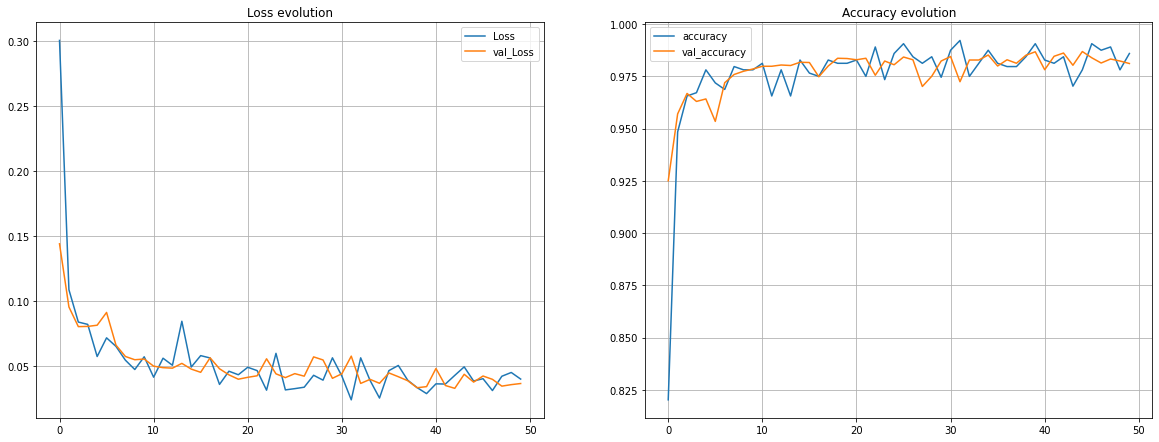
\includegraphics[scale = 0.38]{fileanh/30.png}
        \caption{kết quả train của Model VGG19}
    \end{figure}
\end{center}
\subsubsection{Đánh giá}
Các giá trị trên ma trận nhầm lẫn:
%\newpage
\begin{center}
    \begin{figure}[!h]
        \centering
        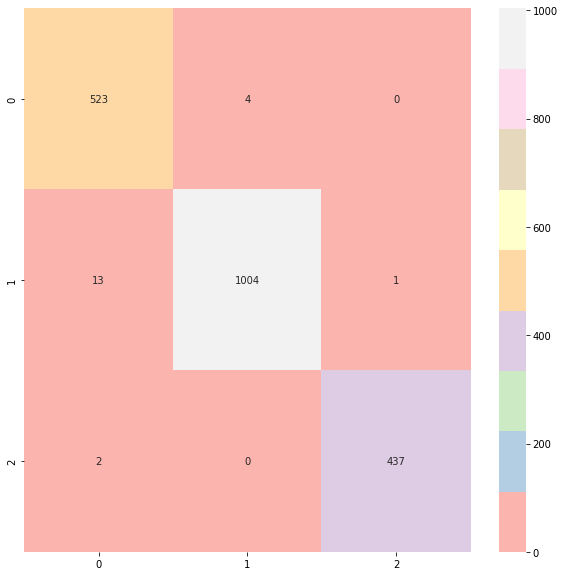
\includegraphics[scale = 0.4]{fileanh/31.png}
        \caption{Confusion matrix của Model VGG19}
    \end{figure}
\end{center}
Và các giá trị Macro average Precision, Macro average Recall, F1-score là:
\begin{center}
    \begin{figure}[!h]
        \centering
        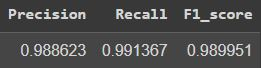
\includegraphics[scale = 1.5]{fileanh/32.jpg}
        \caption{Chỉ số đánh giá của Model VGG19}
    \end{figure}
\end{center}

\subsection{Mô hình 6 - VGG19 với tập dữ liệu lớn}
Sử dụng mô hình VGG19 đã được xây dựng trước đó, thực hiện training với tập dữ liệu lớn hơn.
\subsubsection{Dữ liệu đầu vào }
Bộ dữ liệu đã được tăng cường hình ảnh từ nhiều nguồn khác với tất cả 79596 hình ảnh cho 3 lớp.

\subsubsection{Kết quả training}
\begin{center}
    \begin{figure}[!h]
        \centering
        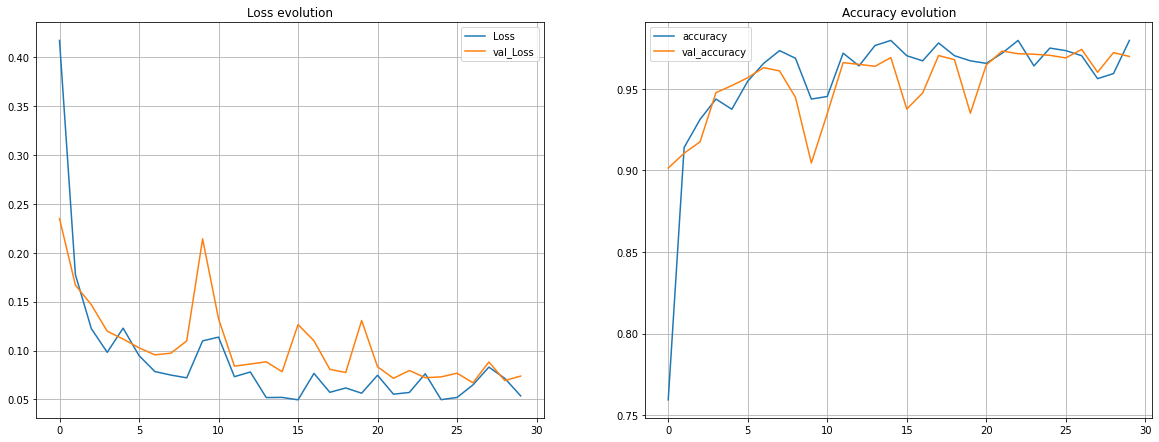
\includegraphics[scale = 0.38]{fileanh/vgg19_increase.png}
        \caption{Kết quả train của Model VGG19 với tập dữ liệu lớn}
    \end{figure}
\end{center}
\subsubsection{Đánh giá}
Ta có ma trận nhầm lẫn như sau:
\begin{center}
    \begin{figure}[!h]
        \centering
        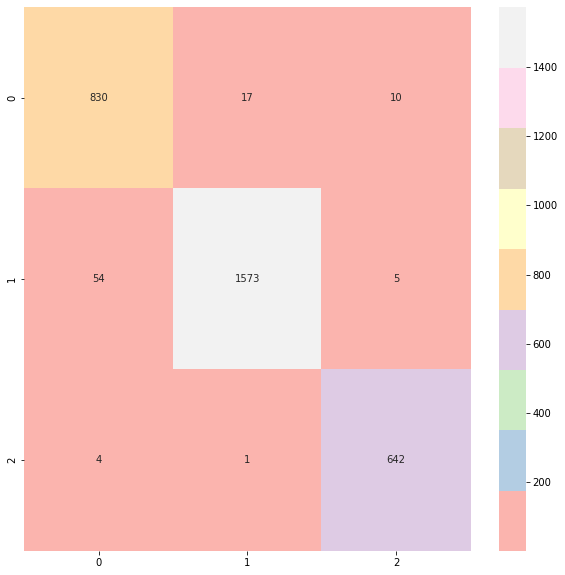
\includegraphics[scale = 0.4]{fileanh/vgg19_increase1.png}
        \caption{Confusion matrix của Model VGG19 với tập dữ liệu lớn}
    \end{figure}
\end{center}
\newpage
Và các giá trị Macro average Precision, Macro average Recall, F1-score là:
\begin{center}
    \begin{figure}[!h]
        \centering
        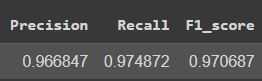
\includegraphics[scale = 1.2]{fileanh/vgg19_increase2.jpg}
        \caption{Các chỉ số đánh giá của Model VGG19 với tập dữ liệu lớn}
    \end{figure}
\end{center}






\subsection{Mô hình 7 - Alexnet}
\subsubsection{Dữ liệu đầu vào}
Bộ dữ liệu \textbf{Fashion Product Images (Small)} đã được xử lý với 41906 hình ảnh cho 3 lớp.
\subsubsection{Xây dựng mô hình}
\begin{lstlisting}
model=Sequential()
model.add(Conv2D(filters=96,strides=(4,4),kernel_size=(11,11),padding='valid',input_shape=(227,227,3),activation='relu'))
model.add(BatchNormalization())
model.add(MaxPooling2D(pool_size=(3,3),strides=(2,2)))
model.add(Conv2D(filters=256,strides=(1,1),kernel_size=(5,5),padding='valid',activation='relu'))
model.add(MaxPooling2D(pool_size=(3,3),strides=(2,2)))
model.add(Conv2D(filters=384,kernel_size=(3,3),strides=(1,1),padding='valid',activation='relu'))
model.add(BatchNormalization())
model.add(Conv2D(filters=384,kernel_size=(3,3),strides=(1,1),padding='valid',activation='relu'))
model.add(BatchNormalization())
model.add(Conv2D(filters=256,kernel_size=(3,3),strides=(1,1),padding='valid',activation='relu'))
model.add(BatchNormalization())
model.add(MaxPooling2D(pool_size=(3,3),strides=(2,2),padding='valid'))
model.add(Flatten())
model.add(Dense(units=4096,activation='relu'))
model.add(Dropout(0.2))
model.add(Dense(units=4096,activation='relu'))
model.add(Dropout(0.2))
model.add(Dense(units=3,activation='softmax')) 
\end{lstlisting}

\begin{lstlisting}
model.compile(loss='binary_crossentropy', optimizer='adam', metrics=['accuracy']) 
alexnet_model=model.fit(training_generator,epochs=50,validation_data=validation_generator,steps_per_epoch=len(training_generator),validation_steps=len(validation_generator))
\end{lstlisting}

\begin{center}
    \begin{figure}[!h]
        \centering
        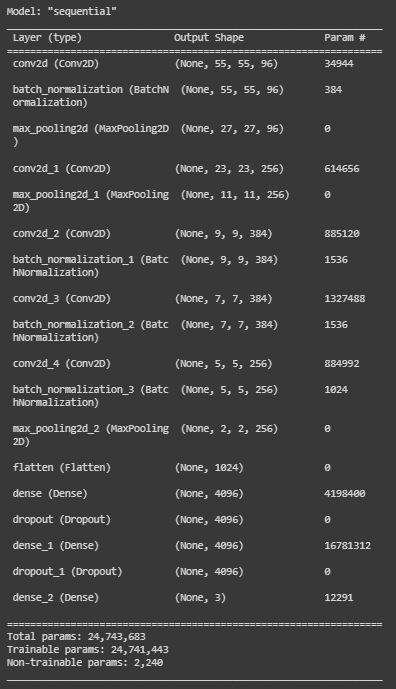
\includegraphics[scale = 1.05]{fileanh/33.jpg}
        \caption{Model Alexnet}
    \end{figure}
\end{center}



\subsubsection{Kết quả training}\newpage
\begin{center}
    \begin{figure}[!h]
        \centering
        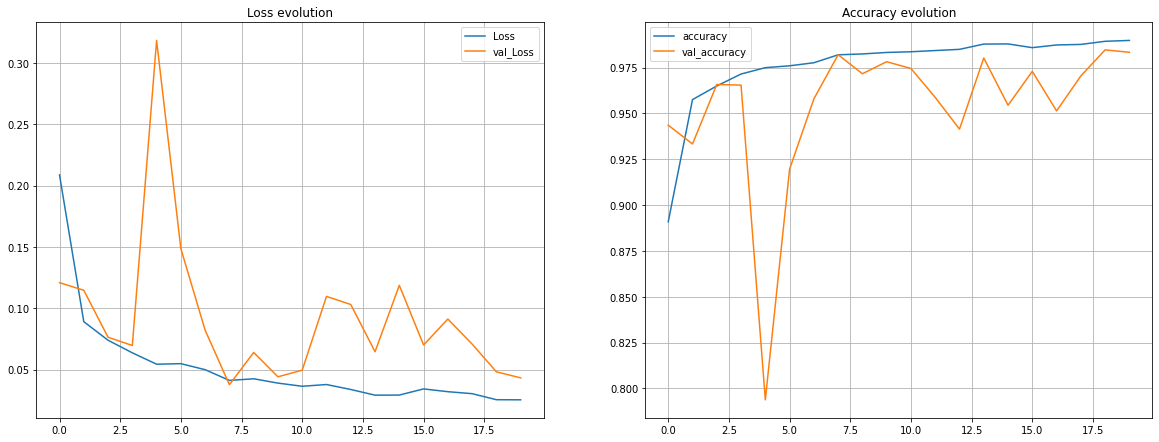
\includegraphics[scale = 0.37]{fileanh/Alexnet.png}
        \caption{kết quả train của Model Alexnet}
    \end{figure}
\end{center}
\subsubsection{Đánh giá}
Các giá trị trên ma trận nhầm lẫn:
%\newpage
\begin{center}
    \begin{figure}[!h]
        \centering
        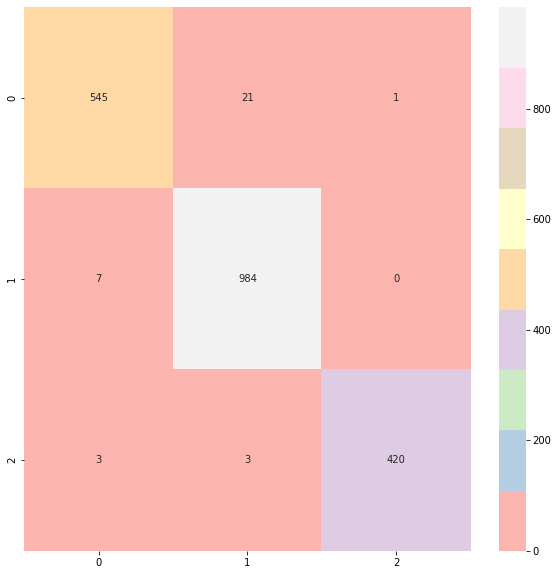
\includegraphics[scale = 0.38]{fileanh/Alexnet1.png}
        \caption{Confusion matrix của Model Alexnet}
    \end{figure}
\end{center}
Và các giá trị Macro average Precision, Macro average Recall, F1-score là:
\begin{center}
    \begin{figure}[!h]
        \centering
        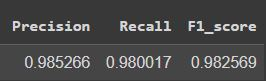
\includegraphics[scale = 1.2]{fileanh/Alexnet2.jpg}
        \caption{Chỉ số đánh giá của Model Alexnet}
    \end{figure}
\end{center}


\subsection{Mô hình 8 - Resnet101}
\subsubsection{Dữ liệu đầu vào}
Bộ dữ liệu \textbf{Fashion Product Images (Small)} đã được xử lý với 41906 hình ảnh cho 3 lớp.
\subsubsection{Xây dựng mô hình}
\begin{lstlisting}
image_size=[227,227]
model=ResNet101(input_shape=image_size+[3],include_top=False,weights="imagenet")
\end{lstlisting}
\begin{lstlisting}
for layers in model.layers:
  layers.trainable=False
\end{lstlisting}
Thêm một số layers cần thiết
\begin{lstlisting}
final_model=Model(inputs=model.input,outputs=Dense(3,activation="softmax")(Flatten()(model.output)))
final_model.summary()
\end{lstlisting}

\begin{center}
    \begin{figure}[!h]
        \centering
        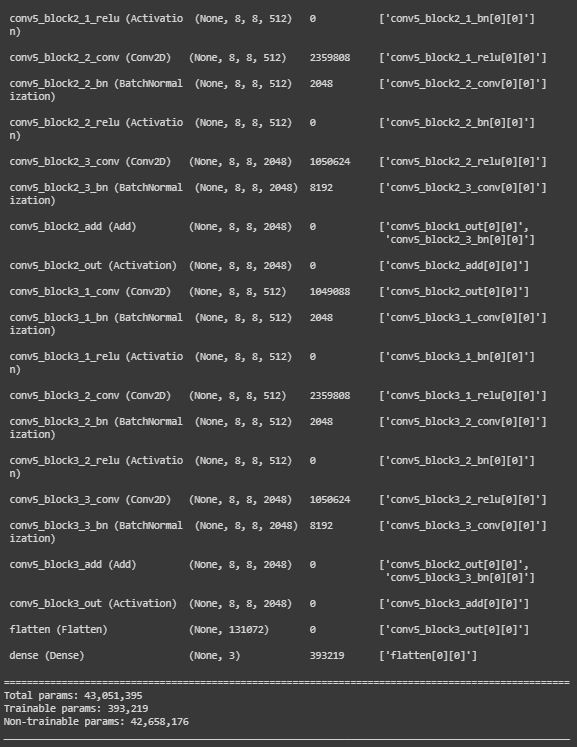
\includegraphics[scale = 0.9]{fileanh/37.jpg}
        \caption{Model Resnet101}
    \end{figure}
\end{center}

\begin{lstlisting}
from tensorflow.keras.optimizers import RMSprop
final_model.compile(loss="categorical_crossentropy",optimizer=RMSprop(lr=0.001),metrics=['accuracy'])
resnet = final_model.fit(training_generator,epochs=50,steps_per_epoch=20,validation_data=validation_generator)
\end{lstlisting}

\subsubsection{Kết quả training}
\begin{center}
    \begin{figure}[!h]
        \centering
        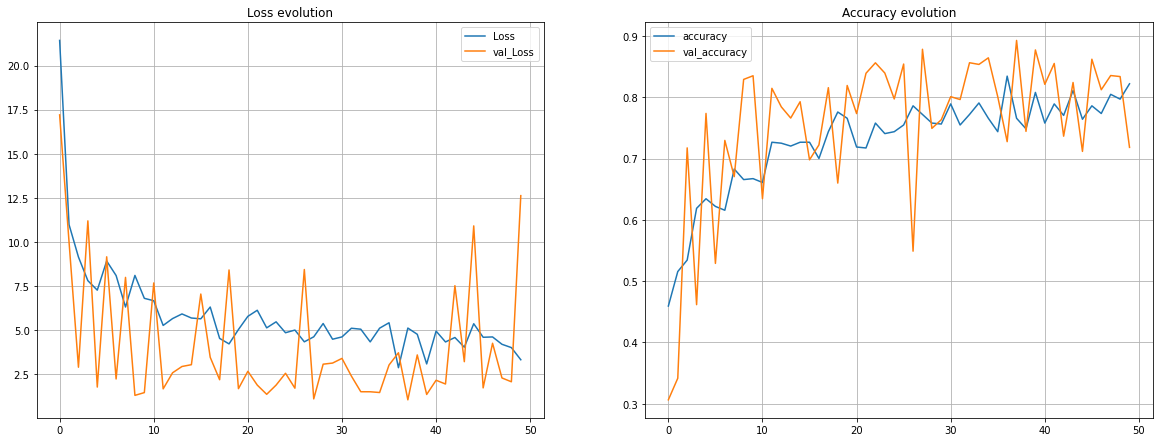
\includegraphics[scale = 0.38]{fileanh/Resnet.png}
        \caption{kết quả train của Model Resnet101}
    \end{figure}
\end{center}
\subsubsection{Đánh giá}
Các giá trị trên ma trận nhầm lẫn:
%\newpage
\begin{center}
    \begin{figure}[!h]
        \centering
        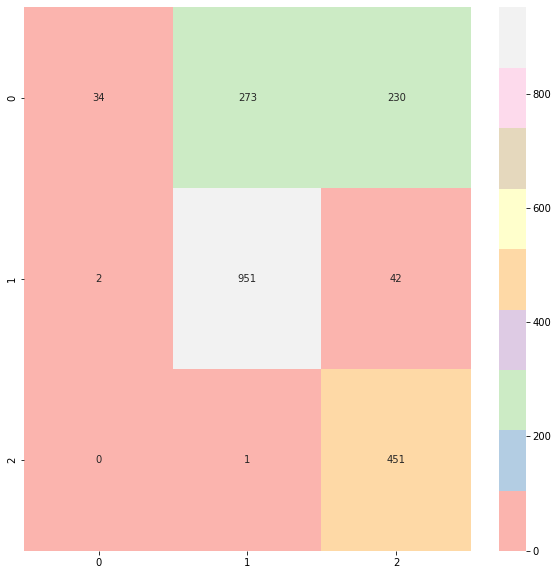
\includegraphics[scale = 0.38]{fileanh/Resnet1.png}
        \caption{Confusion matrix của Model Resnet101}
    \end{figure}
\end{center}
Và các giá trị Macro average Precision, Macro average Recall, F1-score là:
\begin{center}
    \begin{figure}[!h]
        \centering
        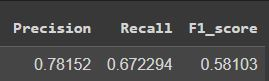
\includegraphics[scale = 1.2]{fileanh/Resnet2.jpg}
        \caption{Chỉ số đánh giá của Model Resnet101}
    \end{figure}
\end{center}

\subsection{Mô hình 9 - Resnet101 với tập dữ liệu lớn}
\subsubsection{Dữ liệu đầu vào }
Bộ dữ liệu đã được tăng cường hình ảnh từ nhiều nguồn khác với tất cả 79596 hình ảnh cho 3 lớp.

\subsubsection{Xây dựng mô hình}
\begin{itemize}
    \item Sử dụng mô hình Resnet101 đã được xây dựng trước đó để thực hiện training với tập dữ liệu lớn hơn.

    \item Đồng thời thực hiện một số thay đổi như sau:
    \begin{itemize}
        \item loss: "categorical\_crossentropy" $\rightarrow$ "binary\_crossentropy"
        
        \item optimizer: RMSprop(lr=0.001) $\rightarrow$ "adam"
    \end{itemize}
    
\end{itemize}
\begin{lstlisting}
final_model.compile(loss="binary_crossentropy",optimizer="adam",metrics=['accuracy'])
\end{lstlisting}


\subsubsection{Kết quả training}
\begin{center}
    \begin{figure}[!h]
        \centering
        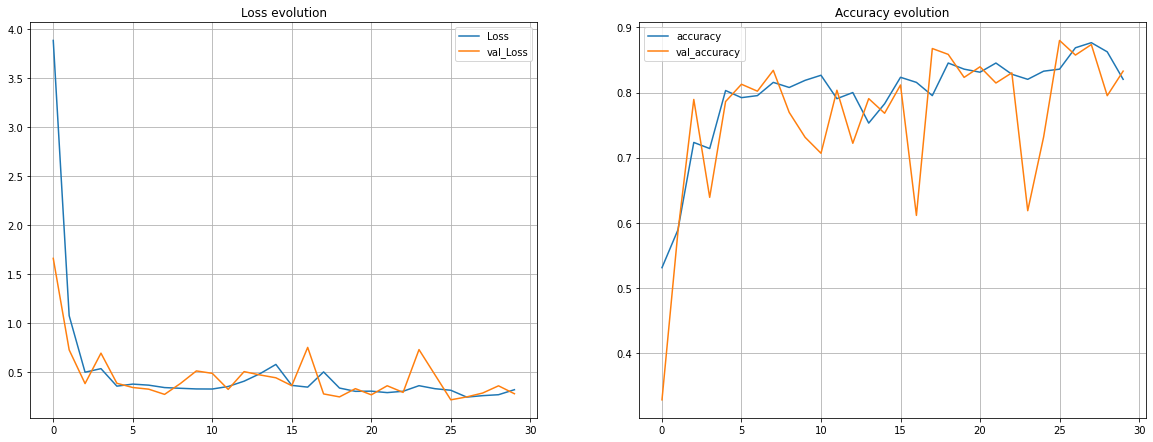
\includegraphics[scale = 0.38]{fileanh/Resnet_increase.png}
        \caption{Kết quả train của Model Resnet101 với tập dữ liệu lớn}
    \end{figure}
\end{center}
\subsubsection{Đánh giá}
Ta có ma trận nhầm lẫn như sau:
\begin{center}
    \begin{figure}[!h]
        \centering
        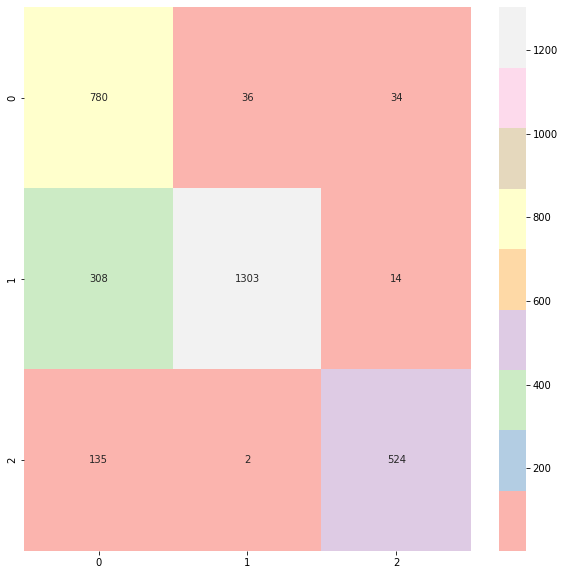
\includegraphics[scale = 0.4]{fileanh/Resnet_increase1.png}
        \caption{Confusion matrix của Model Resnet101 với tập dữ liệu lớn}
    \end{figure}
\end{center}

Và các giá trị Macro average Precision, Macro average Recall, F1-score là:
\begin{center}
    \begin{figure}[!h]
        \centering
        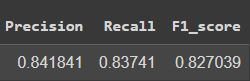
\includegraphics[scale = 1.2]{fileanh/Resnet_increase2.jpg}
        \caption{Các chỉ số đánh giá của Model Resnet101 với tập dữ liệu lớn}
    \end{figure}
\end{center}


\subsection{Mô hình 10 - EfficientNetV2L}
\subsubsection{Dữ liệu đầu vào}
Bộ dữ liệu đã được tăng cường hình ảnh từ nhiều nguồn khác với tất cả 79596 hình ảnh cho 3 lớp.
\subsubsection{Xây dựng mô hình}
\begin{lstlisting}
image_size=[224,224]
model=EfficientNetV2L(input_shape=image_size+[3],include_top=False,weights="imagenet")
\end{lstlisting}
\begin{lstlisting}
for layers in model.layers:
  layers.trainable=False
\end{lstlisting}
Thêm một số layers cần thiết
\begin{lstlisting}
from pandas.core.common import flatten
model=Model(inputs=model.input,outputs=Dense(3,activation="softmax")(Dropout(0.2)(Flatten()(model.output))))
final_model.summary()
\end{lstlisting}

\begin{center}
    \begin{figure}[!h]
        \centering
        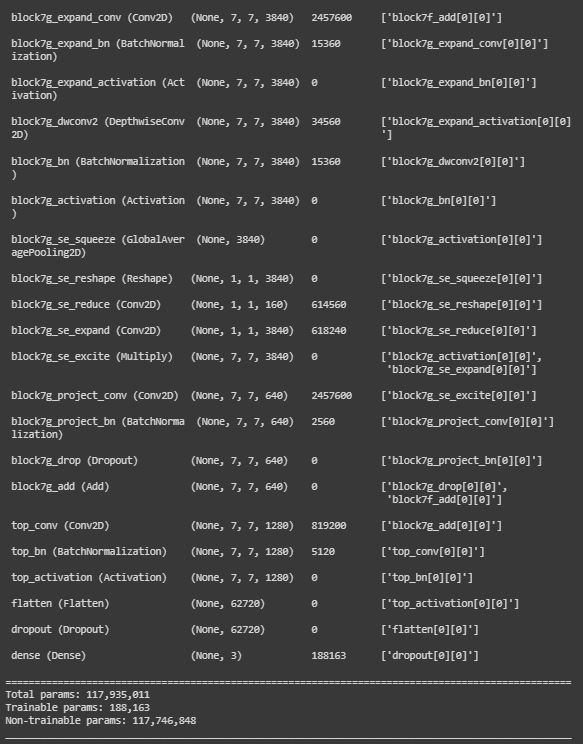
\includegraphics[scale = 1.1]{fileanh/efficient3.jpg}
        \caption{Model EfficientNetV2L}
    \end{figure}
\end{center}

\begin{lstlisting}
model.compile(loss="binary_crossentropy",optimizer="adam",metrics=['accuracy'])
efficientNetV2L = model.fit(training_generator,epochs=30,steps_per_epoch=20,validation_data=validation_generator)
\end{lstlisting}

\subsubsection{Kết quả training}\newpage
\begin{center}
    \begin{figure}[!h]
        \centering
        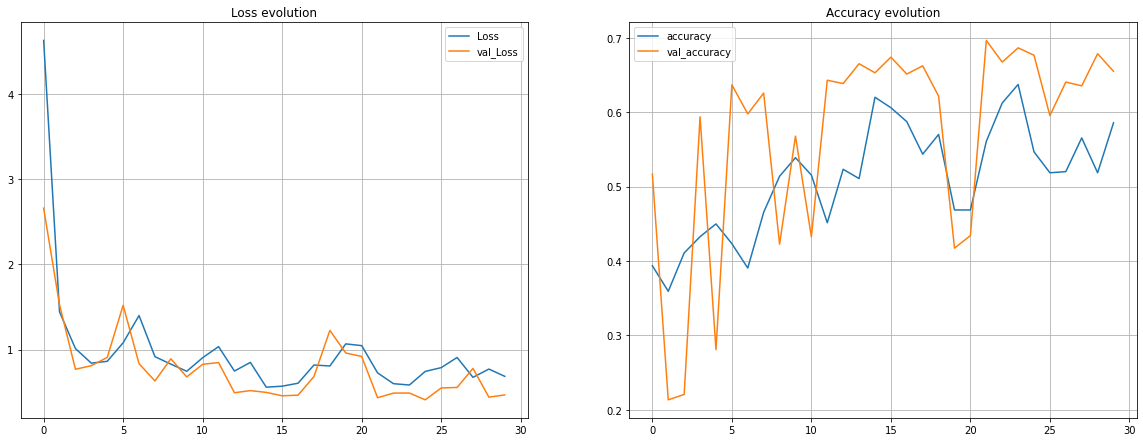
\includegraphics[scale = 0.38]{fileanh/efficient.png}
        \caption{kết quả train của Model EfficientNetV2L}
    \end{figure}
\end{center}
\subsubsection{Đánh giá}
Các giá trị trên ma trận nhầm lẫn:
%\newpage
\begin{center}
    \begin{figure}[!h]
        \centering
        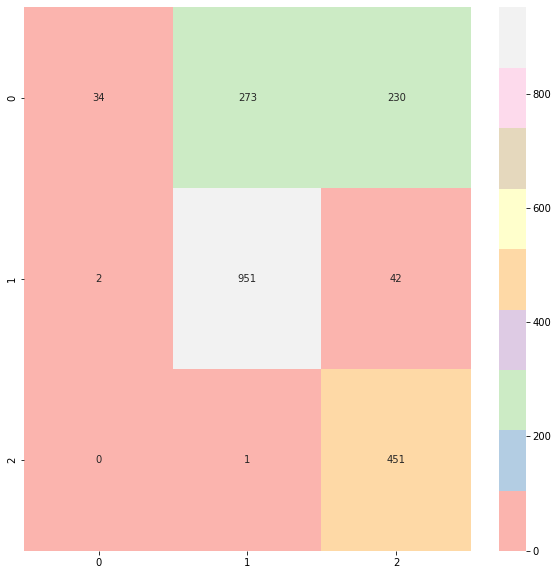
\includegraphics[scale = 0.38]{fileanh/Resnet1.png}
        \caption{Confusion matrix của Model EfficientNetV2L}
    \end{figure}
\end{center}
Và các giá trị Macro average Precision, Macro average Recall, F1-score là:
\begin{center}
    \begin{figure}[!h]
        \centering
        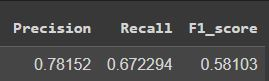
\includegraphics[scale = 1.2]{fileanh/Resnet2.jpg}
        \caption{Chỉ số đánh giá của Model EfficientNetV2L}
    \end{figure}
\end{center}




    